
\subsection{Motivation}
Previous discussion, while giving certain applications of the Sum-Check
protocol, still provides quite ``artificial'' constructions not 
directly applicable in the real-world use-cases. For instance, 
the \#SAT problem is not very practical as the prover $\mathcal{P}$
cannot even compute the value $H$ in polynomial time. Ideally,
we would like to have a protocol that allows the prover to compute
the value $H$ is the polynomial time, while the verifier $\mathcal{V}$
should be able to verify the correctness of the claimed value
$H$ in the logarithmic time. 

Goldwasser, Kalai, and Rothblum (GKR) \cite{gkr} described a protocol which
solves exactly this issue over the arithmetical circuits, which
we solved using QAP$\to$NILP reduction in Groth16. Here we take
the Sum-Check approach.

Suppose we are given the \textit{layered} arithmetical
circuit $\mathtt{C}: \mathbb{F}^n \to \mathbb{F}^m$ of size 
$S$ (number of gates). The \textit{layered} here means 
that the circuit $\mathtt{C}$ can be decomposed into $d$ 
layers (note that GKR can be generalized to the unstructured 
arithmetical circuits as well). The GKR protocol allows 
to achieve the following performance:
\begin{itemize}
    \item The communication consists of $\mathcal{O}(d \cdot \mathsf{polylog}(S))$ field elements.
    \item The verifier runs in $\mathcal{O}(n + d \cdot \mathsf{polylog}(S))$ time.
    \item The prover runs in $\mathcal{O}(\mathsf{poly}(S))$ time.
    \item The soundness error is just $\mathcal{O}(d \log(S) / |\mathbb{F}|)$.
\end{itemize}

\subsection{Protocol Description}

\subsubsection{Circuit Representation}

Again, assume we are given the circuit $\mathtt{C}: \mathbb{F}^n \to
\mathbb{F}^m$ of size $S$, depth $d$, and fan-in two (i.e., each gate has at
most two inputs, but might have multiple outputs). Let us number the layers of
the circuit from $0$ to $d$ where $0$ denotes the output layer while $d$ is the
input layer (notice that the layers are numbered in the reverse order compared
to the usual circuit notation). Assume the number of gates in the layer $i$ is
$S_i$ and without the loss of generality, we assume that $S_i$ is the power of
two: $S_i = 2^{v_i}$. Now, we are going to introduce certain functions 
to further build up the Sum-Check.

\textbf{Gates Encodings.} Suppose $W_i: \{0,1\}^{v_i} \to \mathbb{F}$ is
structured so that it outputs the value of the $i$-th layer gate given the gate
label. As usual, we denote the multilinear extension of $W_i$ as
$\widetilde{W}_i: \mathbb{F}^{v_i} \to \mathbb{F}$.

\textbf{Wiring Predicates.} We introduce the wiring predicates
$\mathsf{in}_{1,i}, \mathsf{in}_{2,i}: \{0,1\}^{v_i} \to \{0,1\}^{v_{i+1}}$
which indicate which pairs of wairing are connected to the $i$-th layer gate
from the layer $i+1$. It takes the label of the gate in the layer $i$ (say, $a$)
and the function $\mathsf{in}_{1,i}(a)$ outputs the label of the first input
connected to the gate $a$ in the layer $i+1$, while $\mathsf{in}_{2,i}(a)$
outputs the label of the second input connected to the gate $a$ in the layer
$i+1$.

\textbf{Operations Encodings.} Define two functions: $\mathsf{add},\mathsf{mul}:
\{0,1\}^{v_i+2v_{i+1}} \to \{0,1\}$ which take three gate labels (say,
$(a,b,c)$) and return $1$ if and only if $(b,c)=(\mathsf{in}_{1,i}(a),
\mathsf{in}_{2,i}(a))$ (that is, the gate $a$ in the layer $i$ is connected to
the gates $b$ and $c$ in the layer $i+1$) and $a$ is an addition gate.
Similarly, $\mathsf{mul}(a,b,c)$ returns $1$ if and only if
$(b,c)=(\mathsf{in}_{1,i}(a), \mathsf{in}_{2,i}(a))$ and $a$ is a multiplication
gate. We denote the MLEs of these functions as $\widetilde{\mathsf{add}}$ and
$\widetilde{\mathsf{mul}}: \mathbb{F}^{v_i+2v_{i+1}} \to \mathbb{F}$,
respectively.

\textbf{Example.} Consider the following circuit with $d=3$ layers:

\begin{figure}[H]

\centering

\resizebox{.9\textwidth}{!}{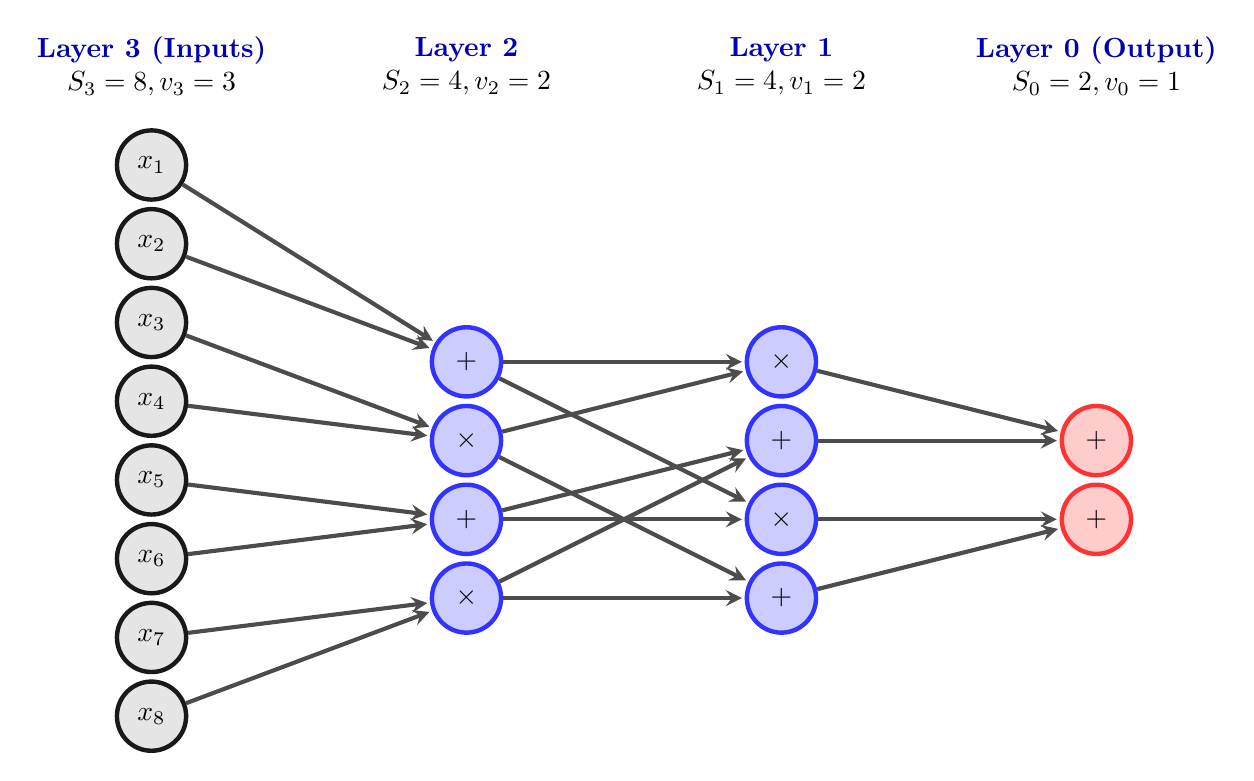
\begin{tikzpicture}[
    % Define styles for different parts of the circuit
    input/.style={circle, ultra thick, draw=gray!20!black, fill=gray!20, minimum size=25pt, inner sep=0pt},
    gate/.style={circle, ultra thick, draw=blue!80, fill=blue!20, minimum size=25pt, inner sep=0pt},
    output/.style={circle, ultra thick, draw=red!80, fill=red!20, minimum size=25pt, inner sep=0pt},
    conn/.style={-stealth, draw=black!70, shorten >=1pt, line width=1.5pt}
]

% --- Layer Labels ---
\node[font=\bfseries, align=center] at (0, 7.75) {\textcolor{blue!70!black}{Layer 3 (Inputs)} \\ $S_3=8,v_3=3$};
\node[font=\bfseries, align=center] at (4, 7.75) {\textcolor{blue!70!black}{Layer 2}\\ $S_2=4,v_2=2$};
\node[font=\bfseries, align=center] at (8, 7.75) {\textcolor{blue!70!black}{Layer 1} \\ $S_1=4,v_1=2$};
\node[font=\bfseries, align=center] at (12, 7.75) {\textcolor{blue!70!black}{Layer 0 (Output)} \\ $S_0=2, v_0=1$};


% --- Layer 0: Input Nodes (8) ---
% We use a \foreach loop to create the 8 input nodes vertically
\foreach \i in {1,...,8} {
    \node[input] (l0-\i) at (0, 7.5 - \i) {$x_{\i}$};
}

% --- Layer 1: Gate Nodes (4) ---
% Alternating between + and x gates
\node[gate] (l1-1) at (4, 4) {$+$};
\node[gate] (l1-2) at (4, 3) {$\times$};
\node[gate] (l1-3) at (4, 2) {$+$};
\node[gate] (l1-4) at (4, 1) {$\times$};

% --- Layer 2: Gate Nodes (4) ---
\node[gate] (l2-1) at (8, 4) {$\times$};
\node[gate] (l2-2) at (8, 3) {$+$};
\node[gate] (l2-3) at (8, 2) {$\times$};
\node[gate] (l2-4) at (8, 1) {$+$};

% --- Layer 3: Output Nodes (2) ---
\node[output] (l3-1) at (12, 3) {$+$};
\node[output] (l3-2) at (12, 2) {$+$};


% --- Connections ---

% Connections from Layer 0 to Layer 1
\foreach \i in {1,...,4} {
    \pgfmathtruncatemacro{\j}{2 * \i - 1} % Calculate first source node index
    \pgfmathtruncatemacro{\k}{2 * \i}     % Calculate second source node index
    \draw[conn] (l0-\j) -- (l1-\i);
    \draw[conn] (l0-\k) -- (l1-\i);
}

% Connections from Layer 1 to Layer 2
% This wiring pattern creates a mixing of the signals
\draw[conn] (l1-1) -- (l2-1);
\draw[conn] (l1-2) -- (l2-1);

\draw[conn] (l1-3) -- (l2-2);
\draw[conn] (l1-4) -- (l2-2);

\draw[conn] (l1-1) -- (l2-3);
\draw[conn] (l1-3) -- (l2-3);

\draw[conn] (l1-2) -- (l2-4);
\draw[conn] (l1-4) -- (l2-4);

% Connections from Layer 2 to Layer 3
\draw[conn] (l2-1) -- (l3-1);
\draw[conn] (l2-2) -- (l3-1);

\draw[conn] (l2-3) -- (l3-2);
\draw[conn] (l2-4) -- (l3-2);

\end{tikzpicture}}
\caption{Example of a layered arithmetical circuit $\mathtt{C}: \mathbb{F}^8 \to
\mathbb{F}^2$ with $d=3$ layers.}
\end{figure}

Let us assume that we have inputted the values $\mathbf{x}^{\langle 3 \rangle} =
(1, 2, 0, 1, 0, 2, 0, 1)$. Then, the value of the layer 2 is
$\mathbf{x}^{\langle 2 \rangle} = (3,0,2,0)$ and the layer 1 is
$\mathbf{x}^{\langle 1 \rangle} = (0, 2, 6, 0)$. Finally, the output layer is
$\mathbf{x}^{\langle 0 \rangle} = (2, 6)$. Let us now see how to encode gates,
wiring predicates, and operations encodings on this circuit. Consider 
$W_1: \{0,1\}^2 \to \mathbb{F}$. We have
\begin{equation*}
    W_1(0, 0) = 0, \quad W_1(0, 1) = 2, \quad W_1(1, 0) = 6, \quad W_1(1, 1) = 0.
\end{equation*}

Therefore, the multilinear extension of $W_1$ is $\widetilde{W}_1(X_1,X_2) =
2(1-X_1)X_2 + 6X_1(1-X_2)$.

Now, let us define the wiring predicates $\mathsf{in}_{1,2}, \mathsf{in}_{2,2}:
\{0,1\}^2 \to \{0,1\}^3$. Consider the 2nd gate ($2=(1,0)$) in layer $2$. It is
connected to the 5th and 6th gates in layer $3$ (the input layer). Since
$5=(1,0,1)$ and $6=(1,1,0)$ in the binary form, we have
\begin{equation*}
    \mathsf{in}_{1,2}(1,0) = (1,0,1), \quad \mathsf{in}_{2,2}(1,0) = (1,1,0).
\end{equation*}

Now, consider the operation encodings $\mathsf{add}_2$ and $\mathsf{mul}_2:
\{0,1\}^8 \to \{0,1\}$. The addition gate is non-zero only on the following inputs:
\begin{equation*}
    (\textcolor{blue!80}{(0,0)},\textcolor{gray!20!black}{(0,0,0)},\textcolor{gray!20!black}{(0,0,1)}), 
    \quad 
    (\textcolor{blue!80}{(1,0)},\textcolor{gray!20!black}{(1,0,0)},\textcolor{gray!20!black}{(1,0,1)}).
\end{equation*}

Therefore, the multilinear extension of $\mathsf{add}_2$ is
\begin{align*}
    \widetilde{\mathsf{add}}_2(X_1,X_2,Y_1,Y_2,Y_3,Z_1,Z_2,Z_3) &= (1-X_1)(1-X_2)(1-Y_1)(1-Y_2)\\
    &\cdot (1-Y_3)(1-Z_1)(1-Z_2)Z_3 \\
    &+ X_1(1-X_2)Y_1(1-Y_2)(1-Y_3)Z_1(1-Z_2)Z_3 \\
\end{align*}

Similarly, the multiplication encoding $\mathsf{mul}_2$ is non-zero only on the
following inputs:
\begin{equation*}
    (\textcolor{blue!80}{(0,1)},\textcolor{gray!20!black}{(0,1,0)},\textcolor{gray!20!black}{(0,1,1)}), 
    \quad
    (\textcolor{blue!80}{(1,1)},\textcolor{gray!20!black}{(1,1,0)},\textcolor{gray!20!black}{(1,1,1)}),
\end{equation*}

The multilinear extension of $\mathsf{mul}_2$ is
\begin{align*}
    \widetilde{\mathsf{mul}}_2(X_1,X_2,Y_1,Y_2,Y_3,Z_1,Z_2,Z_3) &= (1-X_1)X_2(1-Y_1)Y_2(1-Y_3)(1-Z_1)Z_2Z_3 \\
    &+ X_1X_2Y_1Y_2(1-Y_3)Z_1Z_2Z_3.
\end{align*}

\begin{remark}
    Note that the operations encodings $\mathsf{add}_i$ and $\mathsf{mul}_i$
    (and thus MLEs $\widetilde{\mathsf{add}}_i$ and
    $\widetilde{\mathsf{mul}}_i$) do not depend on the solution witness
    $\{\mathbf{x}^{\langle i \rangle}\}_{i \in [d+1]}$, while the gates
    encodings $W_i$ do depend.
\end{remark}

\subsubsection{Protocol Specification}

The GKR protocol consists of $d$ rounds, one for each layer of the circuit. In
the $i$-th round, the prover $\mathcal{P}$ claims a value for
$\widetilde{W}_i(\mathbf{r}_i)$ at the randomly selected point $\mathbf{r}_i
\leftarrowS \mathbb{F}^{v_i}$. 

At the start of the 1st round, this claim is made about the circuit outputs.
Namely, if we have $S_0=2^{v_0}$ gates in the output layer, let $D:
\{0,1\}^{v_0} \to \mathbb{F}$ denote the function which maps the gate label to
the claimed output value, sent by the prover $\mathcal{P}$. The verifier picks a
random point $\mathbf{r}_0 \leftarrowS \mathbb{F}^{v_0}$ and evaluates
$\widetilde{D}(r_0)$ in time $\mathcal{O}(S_0)$. By the Schwartz-Zippel lemma,
if $\widetilde{D}(\mathbf{r}_0)=\widetilde{W}_0(\mathbf{r}_0)$, then with the
soundness error of $v_0/|\mathbb{F}|^{v_0}$ the verifier is assured that these
two polynomials are indeed equal. However, for obvious reasons, the verifier
cannot compute $\widetilde{W}_0(\mathbf{r}_0)$ without the prover's help. So the
core idea of GKR is to reduce the claim about the value of
$\widetilde{W}_i(\mathbf{r}_i)$ to a claim about the value of
$\widetilde{W}_{i+1}(\mathbf{r}_{i+1})$ for some randomly chosen
$\mathbf{r}_{i+1} \leftarrowS \mathbb{F}^{v_{i+1}}$. How? Consider the
following lemma.

\begin{lemma}
    The following statement holds:
    \begin{align*}
        \small\widetilde{W}_i(\mathbf{z}) &= \sum_{\boldsymbol{b},\boldsymbol{c} \in \{0,1\}^{v_{i+1}}} \Big(\widetilde{\mathsf{add}}_i(\mathbf{z},\boldsymbol{a},\boldsymbol{b})(\widetilde{W}_{i+1}(\boldsymbol{b}) + \widetilde{W}_{i+1}(\boldsymbol{c})) \\
        &+ \widetilde{\mathsf{mul}}_i(\mathbf{z},\boldsymbol{b},\boldsymbol{c})\widetilde{W}_{i+1}(\boldsymbol{b})\widetilde{W}_{i+1}(\boldsymbol{c})\Big).
    \end{align*}
\end{lemma}

\textbf{Proof.} Since both sides are multilinear polynomials, it suffices to
check that the equality holds for all boolean assignments $\mathbf{z} \in
\{0,1\}^{v_i}$. Fix some concrete $\mathbf{z}_0 \in \{0,1\}^{v_i}$ and without
the loss of generality, assume that $\mathbf{z}_0$ is the addition gate in the
layer $i$ (the case of multiplication gate is similar). In such case, all 
the terms $\widetilde{\mathsf{mul}}_i(\mathbf{z},\boldsymbol{b},\boldsymbol{c})$ 
will be zero, so we can reduce the sum down to:
\begin{equation*}
    \widetilde{W}_i(\mathbf{z}_0) = \sum_{\boldsymbol{b},\boldsymbol{c} \in \{0,1\}^{v_{i+1}}} \widetilde{\mathsf{add}}_i(\mathbf{z}_0,\boldsymbol{a},\boldsymbol{b})(\widetilde{W}_{i+1}(\boldsymbol{b}) + \widetilde{W}_{i+1}(\boldsymbol{c}))
\end{equation*}

Now, according to the definition of the $\widetilde{\mathsf{add}}_i$ predicate,
the $\widetilde{\mathsf{add}}_i(\mathbf{z}_0,\boldsymbol{b},\boldsymbol{c})$ is
non-zero (equals to $1$) only if $(\boldsymbol{b}, \boldsymbol{c}) =
(\mathsf{in}_{1,i}(\mathbf{z}_0), \mathsf{in}_{2,i}(\mathbf{z}_0))$. Since we
know that $\mathbf{z}_0$ is an addition gate, we can conclude that two such
gates $\boldsymbol{b}$ and $\boldsymbol{c}$ exist. Therefore, we can rewrite the
sum as:
\begin{equation*}
    \widetilde{W}_{i+1}(\mathsf{in}_{1,i}(\mathbf{z}_0)) + \widetilde{W}_{i+1}(\mathsf{in}_{2,i}(\mathbf{z}_0)) = \widetilde{W}_i(\mathbf{z}_0).
\end{equation*}

That said, to check the $\mathcal{P}$'s claim about $\widetilde{W}_i(\mathbf{r}_i)$, the verifier 
can apply the Sum-Check protocol on the function
\begin{equation*}
    f_i(\boldsymbol{b}, \boldsymbol{c}; \mathbf{r}_i) = \widetilde{\mathsf{add}}_i(\mathbf{r}_i, \boldsymbol{b}, \boldsymbol{c})(\widetilde{W}_{i+1}(\boldsymbol{b}) + \widetilde{W}_{i+1}(\boldsymbol{c})) + \widetilde{\mathsf{mul}}_i(\mathbf{r}_i, \boldsymbol{b}, \boldsymbol{c})\widetilde{W}_{i+1}(\boldsymbol{b})\widetilde{W}_{i+1}(\boldsymbol{c}).
\end{equation*}

However, note that \textit{the verifier $\mathcal{V}$ does not know the
polynomial $\widetilde{W}_{i+1}$}. However, note that he does not need to know
it until the last round, during which $\mathcal{V}$ has to make the oracle
request $\mathcal{O}^{f_i}$ to compute the value of $f_i$ at the randomly
selected point $(\boldsymbol{b}^*, \boldsymbol{c}^*) \leftarrowS
\mathbb{F}^{2v_{i+1}}$. Evaluating $f_i(\boldsymbol{b}^*, \boldsymbol{c}^*;
\mathbf{r}_i)$ requires evaluating
$\widetilde{\mathsf{add}}_i(\mathbf{r}_i,\boldsymbol{b}^*,\boldsymbol{c}^*)$,
$\widetilde{\mathsf{mul}}_i(\mathbf{r}_i,\boldsymbol{b}^*,\boldsymbol{c}^*)$,
and $\widetilde{W}_{i+1}(\boldsymbol{b}^*)$ with
$\widetilde{W}_{i+1}(\boldsymbol{c}^*)$. Note that evaluating the first two
terms can be done by the verifier $\mathcal{V}$ in
$\mathcal{O}(\mathsf{poly}(v_i,v_{i+1}))$. However, evaluating the last two
terms requires the prover $\mathcal{P}$ to assist the verifier. So we are going
to do the following: the prover $\mathcal{P}$ sends the values
$z_b=\widetilde{W}_{i+1}(\boldsymbol{b}^*)$ and
$z_c=\widetilde{W}_{i+1}(\boldsymbol{c}^*)$ to the verifier $\mathcal{V}$. Now
the verifier has to check both these values are correct. However, here is the
issue: during the sum-check protocol, the verifier can only use a single random
point $\mathbf{r}_{i+1} \in \mathbb{F}^{v_{i+1}}$. So how do we check both 
conditions using one random point? Here is the trick.

\begin{proposition}
    Let $\ell: \mathbb{F} \to \mathbb{F}^{v_{i+1}}$ be the line such that
    $\ell(0)=\boldsymbol{b}^*$ and $\ell(1)=\boldsymbol{c}^*$. Then, the prover
    $\mathcal{P}$ sends the univariate polynomial $q(X)$ claimed to be equal to
    $\widetilde{W}_{i+1} \circ \ell$ --- the restriction of
    $\widetilde{W}_{i+1}$ to the line $\ell$. $\mathcal{V}$ checks whether
    indeed $\ell(0)=z_b$ and $\ell(1)=z_c$, then chooses a random point
    $\mathbf{r}^* \leftarrowS \mathbb{F}^{v_{i+1}}$ and checks whether
    $\widetilde{W}_{i+1}(\ell(\mathbf{r}^*)) = q(\mathbf{r}^*)$.
\end{proposition}

This way, the interaction between the prover and the verifier at this round ends
with the new claim about the value of $\widetilde{W}_{i+1}(\mathbf{r}_{i+1})$
with $\mathbf{r}_{i+1} := \ell(\mathbf{r}^*)$.

Finally, we need to define the last round of the protocol. Here, 
the $\mathcal{V}$ simply evaluates $\widetilde{W}_d(\mathbf{r}_d)$
on his own, costing $\mathcal{O}(n)$ time. 

\begin{proposition}
We finally summarize the GKR protocol:
\begin{itemize}
    \item At the start of the first round, $\mathcal{P}$ sends a function 
    $D: \{0,1\}^{v_0} \to \mathbb{F}$ claimed to equal $W_0$ (that is, he 
    essentially sends the values of the output layer gates).
    \item $\mathcal{V}$ picks a random point $\mathbf{r}_0 \leftarrowS
    \mathbb{F}^{v_0}$ and finds $m_0 \gets \widetilde{D}(\mathbf{r}_0)$.
    \item For each $i \in [d]$ we do the following:
    \begin{itemize}
        \item Define the $2v_i$-variate polynomial:
        \begin{align*}
            f_i(\boldsymbol{b}, \boldsymbol{c}; \mathbf{r}_i) &= \widetilde{\mathsf{add}}_i(\mathbf{r}_i, \boldsymbol{b}, \boldsymbol{c})(\widetilde{W}_{i+1}(\boldsymbol{b}) + \widetilde{W}_{i+1}(\boldsymbol{c})) \\
            &+ \widetilde{\mathsf{mul}}_i(\mathbf{r}_i, \boldsymbol{b}, \boldsymbol{c})\widetilde{W}_{i+1}(\boldsymbol{b})\widetilde{W}_{i+1}(\boldsymbol{c}).
        \end{align*}
        \item $\mathcal{P}$ sends the value $m_i$ claimed to equal
        $\sum_{\boldsymbol{b}, \boldsymbol{c} \in
        \{0,1\}^{v_{i+1}}}f_i(\boldsymbol{b}, \boldsymbol{c}; \mathbf{r}_i)$.
        \item $\mathcal{V}$ applies the Sum-Check protocol on the function
        $f_i(\cdot; \mathbf{r}_i)$ up until the last round, where the
        $\mathcal{V}$ has to compute the value $f_i(\boldsymbol{b}^*,
        \boldsymbol{c}^*; \mathbf{r}_i)$ at random $(\boldsymbol{b}^*,
        \boldsymbol{c}^*) \in \mathbb{F}^{2v_{i+1}}$.
        \item Both prover and the verifier computes the line $\ell: \mathbb{F} \to
        \mathbb{F}^{v_{i+1}}$ such that $\ell(0)=\boldsymbol{b}^*$ and
        $\ell(1)=\boldsymbol{c}^*$. $\mathcal{P}$ sends the univariate
        polynomial $q(X)$ claimed to equal $\widetilde{W}_{i+1} \circ \ell$.
        \item $\mathcal{V}$ computes the required value $f_i(\boldsymbol{b}^*,
        \boldsymbol{c}^*; \mathbf{r}_i)$ using $q(0)$ and $q(1)$ instead of 
        $\widetilde{W}_{i+1}(\boldsymbol{b}^*)$ and $\widetilde{W}_{i+1}(\boldsymbol{c}^*)$.
        \item $\mathcal{V}$ chooses a random point $\mathbf{r}^* \leftarrowS
        \mathbb{F}^{v_{i+1}}$ and sets $\mathbf{r}_{i+1} \gets
        \ell(\mathbf{r}^*)$ and $m_{i+1} \gets q(\mathbf{r}_{i+1})$.
        \item The check reduces to verifying that
        $\widetilde{W}_{i+1}(\mathbf{r}_{i+1}) = m_{i+1}$, so proceed to the
        next step.
    \end{itemize}
    \item At the last round, $\mathcal{V}$ directly checks whether
    $m_d=\widetilde{W}_d(\mathbf{r}_d)$.
\end{itemize}
\end{proposition}
